\subsection{Sensitivity to the balanced SciFact selection}
\label{sec:scifact3-census}
The preceding 60/60/60 slice deliberately changed the official cited-pair label mix. To test whether its class-conditional reversal signal depends on that selection, we conducted a \emph{post-hoc same-source census}: every one of the 339 eligible development claim--cited-abstract pairs (138 SUPPORT, 71 CONTRADICT, 130 derived NOINFO) received all four three-choice conditions in a fresh run of all five systems. The 159 pairs outside the prior three-choice selection contain 78/11/70 by reference class; they are not an independent holdout, and 37 positive pairs had already appeared in our earlier \emph{two-choice} SciFact task. Claims and documents can recur in the census, so paired 10,000-draw percentile intervals resample claims as the primary cluster and documents as a sensitivity check. The NOINFO reference retains its narrow provenance: an explicitly cited document with no annotated abstract-evidence entry, not an independently re-adjudicated negative.

\begin{table}[H]
\centering\small
\setlength{\tabcolsep}{4pt}
\begin{tabular}{lrrrr}
\toprule
System & Full 339 & Outside 159 & NOINFO 70 & Flips / repeat \\
\midrule
Laya English & 171$\to$164 & 90$\to$88 & 16$\to$13 & 29 / 0 \\
Laya Multilingual & 150$\to$150 & 77$\to$80 & 8$\to$8 & 63 / 0 \\
Llama 3.1 8B & 182$\to$158 & 103$\to$90 & 33$\to$15 & 73 / 0 \\
Qwen3 8B & 231$\to$220 & 129$\to$119 & \textbf{60$\to$38} & 97 / 0 \\
Jev 1.13 & 291$\to$292 & 144$\to$143 & 59$\to$59 & 5 / 4 \\
\bottomrule
\end{tabular}
\caption{Fresh full-census results. Each arrow shows base$\to$joint-reversal reference-correct counts on the stated denominator. ``Outside 159'' means outside the earlier balanced \emph{three-choice} selection, not unseen model data. Flips compare valid semantic labels; repeat is byte-identical to base. All base/reversal outputs were valid; Jev had one invalid title-removal response, retained separately.}
\label{tab:scifact3-census}
\end{table}

\begin{figure}[H]
\centering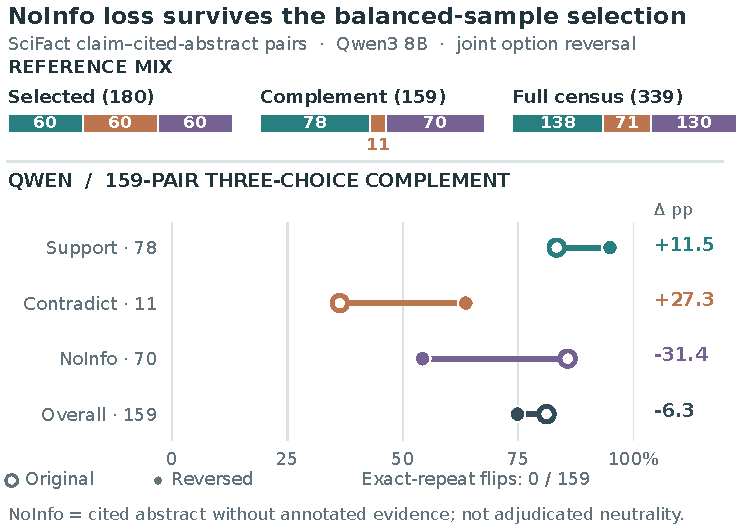
\includegraphics[width=.99\linewidth]{figures/fig_scifact3_census_main.pdf}
\caption{Fresh, post-hoc SciFact cited-pair census sensitivity check. The top strip compares reference-label composition in the selected 180, its 159-pair complement, and all 339 eligible pairs. The lower panel shows Qwen's original (open) and joint-reversal (filled) reference agreement on the complement; differences are percentage points. This is the same source, not an independent holdout: 37 complement positives appeared in the earlier two-choice task. \textsc{NoInfo} is an explicitly cited abstract without annotated evidence, not adjudicated neutrality.}
\label{fig:scifact3-census}
\end{figure}

The earlier Qwen class-opposing pattern persists in the previously unselected three-choice pairs: on their NOINFO references, correctness drops $60\to38/70$ ($-31.4$ points; paired claim-cluster 95\% interval $[-42.4,-21.1]$, document-cluster $[-42.9,-20.3]$), with 22 correct NOINFO decisions migrating to other labels and no reverse corrections into NOINFO. SUPPORT improves $65\to74/78$ and the much smaller CONTRADICT slice $4\to7/11$, leaving the aggregate $129\to119/159$ ($-6.3$ points, claim interval $[-13.7,+1.2]$). On the full 339 pairs, Qwen's NOINFO is $112\to68/130$ ($-33.8$ points, claim interval $[-42.1,-26.0]$), while overall correctness is $231\to220/339$ ($-3.2$ points, $[-8.4,+2.0]$). Its full-census prediction marginal changes from SUPPORT/CONTRADICT/NOINFO $144/11/184$ to $216/33/90$; thus the near-flat aggregate again conceals a substantial answer redistribution. Llama also loses NOINFO correctness on the 159-pair complement ($33\to15/70$, claim interval $[-36.8,-15.7]$), whereas Laya and Jev do not show the same class-specific magnitude (Table~\ref{tab:scifact3-census}). These are joint interface effects, not isolated code or display-order effects.

An identical-request cross-run audit tempers exact-count comparisons with the balanced run. All 720 overlapping request hashes match; for the two local LLMs, every overlapping prompt-token hash matches as well. Nonetheless, Qwen's prior balanced base has two NOINFO decisions that change to SUPPORT in the fresh census run, shifting its selected-subset base count $104\to102/180$; reversal remains $101/180$. The fresh selected-subset NOINFO decline is still $52\to30/60$ (claim interval $[-48.3,-25.0]$), versus $54\to30/60$ previously. Both used batch size four but different co-batches; this audit cannot isolate batching from other numerical or serving variability. We therefore never splice prior selected-subset predictions into the new complement. One Jev \texttt{InvalidDecision} occurred only under title removal; all other census responses were valid. A separate, offline semantic tie-break sensitivity changes full-census reversed correctness only from $158\to159/339$ for Llama and $220\to219/339$ for Qwen; the class-level direction persists, but these ties reinforce that the decoder is part of the evaluated adapter. The census shares the same source and derived-reference limitations as Section~\ref{sec:scifact3}; the title-removal question's reference to an absent title also precludes a clean causal interpretation. Complete confusion matrices, claim/document intervals, case-level predictions, overlap IDs and SHA-256-bound raw outputs are in the companion census artifact.
